\section{ Web-Programmierschnittstelle (Web-API)}
% Einleitung, Motivation
Die Webseite der Wetterstation bietet den interessierten Personen Informationen zum aktuellen Wetter in Arbon. Diese Informationen sind aber nicht nur für Menschen interessant, sondern auch für andere Computer beziehungsweise Server. Das Seebad Arbon zum Beispiel möchte die Wassertemperatur der Wetterstation auf ihrer Webseite anzeigen. Um die Kommunikation von Server zu Server zu vereinfachen werden maschinenlesbare Schnittstellen eingesetzt, sogenannte application programming interfaces (API). Abbildung\,\ref{img:humanvsmachine} zeigt den Unterschied der beiden Darstellungsarten. Auf der linken Seite ist die für den Menschen grafisch mit Farben und Formen aufbereitete Information der Lufttemperatur, auf der rechten Seite die schlichte und rein textbasierte Maschinenversion.

\begin{figure}[htbp!]
  \fbox{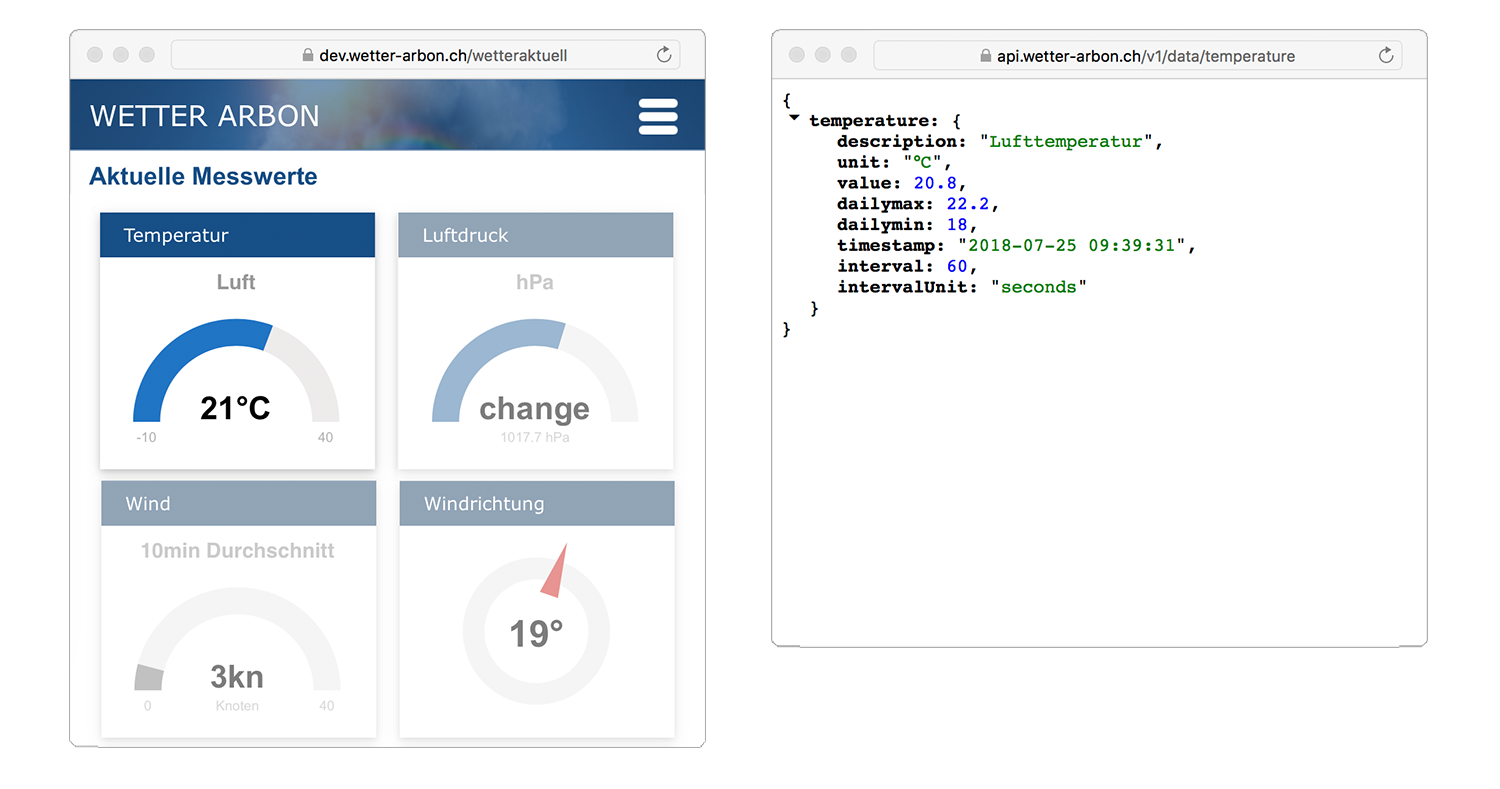
\includegraphics[width=\textwidth-2\fboxsep-2\fboxrule]{img/humanvsmachine}}
	\centering
	\caption{Grafische vs. maschinenlesbare Darstellung}
	\label{img:humanvsmachine}
\end{figure}


Um die API zu entwickeln, wurden die Anforderungen in einen sogenannten Daten-tree (siehe Anhang Listing \ref{lst:JsonTree}) umgeformt. Hieraus wird auch die URL entstehen zur Abfrage der Daten. Der Aufruf wird Grundsätzlich über api.wetter-arbon.ch gemacht. Um einzelne Werte abzufragen muss tiefer in die Verzeichnisse gegangen werden.

\noindent
\url{https://api.wetter-arbon.ch/v1/}\\
\url{https://api.wetter-arbon.ch/v1/data/}\\
\url{https://api.wetter-arbon.ch/v1/data/temperature}\\


%% ############################################################################
%% Unterkapitel
%% ############################################################################
\subsection{Designprinzp (REST) und Hierarchische Struktur}
Die Programmierschnittstelle liefert die aktuellen Messwerte der Wetterstation, Zusatzinformationen, und Infos zur Webcam. Diese Unterteilung wurde bei der Strukturierung der Daten berücksichtigt.
Wie in Abbildung\,\ref{img:hierarchie} ersichtlich, stellt die Versionsnummer den Ausgangspunkt dar. Danach gibt es die drei Untergruppen misc, webcam und data. Unter data werden alle Informationen, die von der Wetterstation direkt oder indirekt gemessen werden angezeigt. Unter webcam ist der Link zu Webcam aufgeführt und unter misc sind die Zusatzinformation die Sturmwinddaten für die drei Region Bodensee Ost, Mittel und West aufgeführt. Die Struktur wurde so gewählt, dass sie logisch ist, sich beliebig erweitern lässt und die URL trotzdem möglichst kurz ist.

\begin{figure}[htbp!]
  \fbox{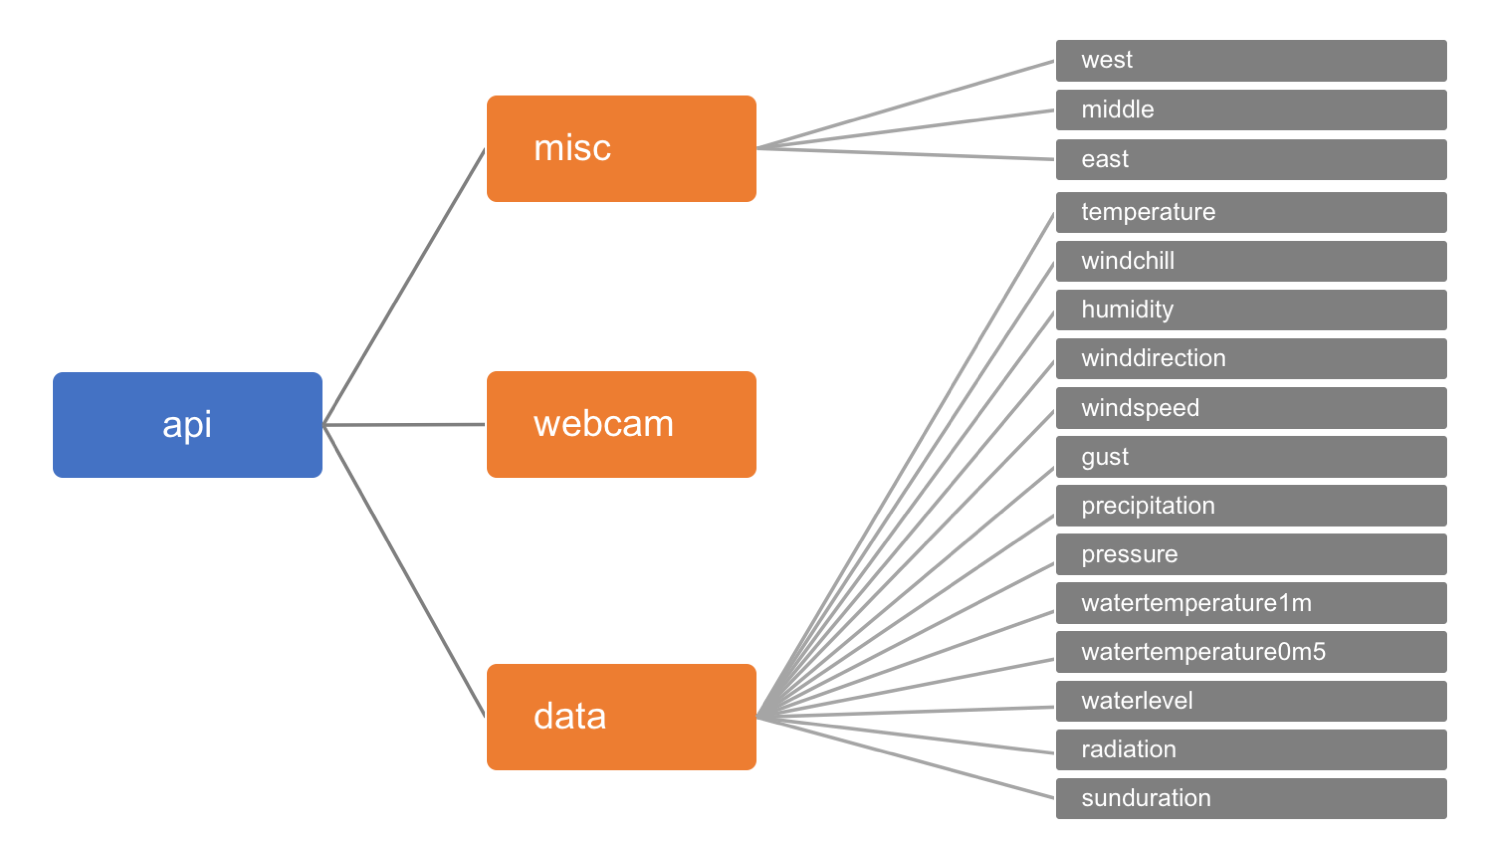
\includegraphics[width=\textwidth-2\fboxsep-2\fboxrule]{img/hierarchie}}
	\centering
	\caption{Dreistufige Datenhierarchie}
	\label{img:hierarchie}
\end{figure}







% REST
Warum REST-Schnittstelle? Was ist der Vorteil gegenüber anderen Schnittstellen? Wie wurden früher Schnittstellen zur Verfügung gestellt?
Was ist REST -> Doktorarbeit von Roy Fielding
Welche Daten sind enthalten
Als nächstes fügen wir der Client-Server-Interaktion eine Einschränkung hinzu: Die Kommunikation muss zustandslos sein, wie in Abschnitt 3.4.3 (Abbildung 5-3), so dass jede Anfrage von Client zu Server alle notwendigen Informationen enthalten muss, um die Anfrage zu verstehen, und keinen auf dem Server gespeicherten Kontext nutzen kann. Der Sitzungszustand bleibt somit vollständig auf dem Client erhalten.
REST ist ein Set von Einschränkungen, der versucht, Latenzzeiten und Netzwerkkommunikation zu minimieren und gleichzeitig die Unabhängigkeit und Skalierbarkeit von Komponentenimplementierungen zu maximieren.
%https://www.ics.uci.edu/~fielding/pubs/dissertation/top.htm
Heutzutage werden viele API nach dem RESTful Standard entwickelt wird. RESt steht für State Transfer und ist im Gegensatz zu Protokollen eine Philosophie, welche die Möglichkeiten von HTTPS ausnutzt. REST benötigt hierfür die von HTTPS bekannten Verben (GET, POST, PUT, PATCH, DELETE) \cite{LornaJaneMitchell2013oreilly}. Im Vordergrund bei REST steht die Zustandslosigkeit, dass heisst Server sowie Client haben keinen Zustand zwischen den Anfragen. Eine Verbindung bleibt jedoch bis zum Ende der Anwendung oder Nutzzeit bestehen.
Die Datenabfrage über die API soll, wie es State of the Art entwickelt wird, RESTful sein und mittels HTTP geschehen. Mit der API werden nur GET-Anfragen erlaubt sein

\noindent
\Diskussionspunkt{Was passiert bei POST-Aufruf?}\newline

% Versionierung
URLs
Versionierung -> semantic Versionierung
1. MAJOR Hauptversion (nicht kompatibel untereinander)
2. MINOR .... (gerade = stabil, ungerade = instabil)
3. PATCH ..... Bug, Patch
Norm?
Versionierung in der URL ermöglich Parallelbetrieb (=Vorteil)
Als nächstes muss ein URL Schema her. Dies wird benötigt, um nach dem REST Standard zu arbeiten. Die URL sollte folgendermassen aussehen:


\\\emph{Protokoll://Host/Versionsnummer/Endpunkt} \\

Die Versionsnummer wird zur Weiterentwicklung benötigt. Wird beispielsweise eine neue Version der API veröffentlicht, kann es sein, dass nicht alle Nutzer der API auf die neue Version umgestiegen sind. Somit kann es geschehen, dass die vorhandenen Installationen zerstört werden.








%% ############################################################################
%% Unterkapitel
%% ############################################################################
\subsection{Rückgabeformat}
JSON vs. XML
Verwendung auf der eigenen Webseite

 Neben der URL ist es wichtig, dass die Kommunikation in einem bestimmten Datenformat erfolgt. Hier besteht die Möglichkeit zu wählen zwischen JSON, XML oder CSV zu wählen. Es können auch andere Formate genutzt werden. Wichtig ist jedoch, dass der Server sowie der Client wissen welches Format genutzt wird. Nebst der Entwicklung für die Server-Client Kommunikation ist auch bei der API eine Zugangskontrolle bzw. eine Grundbasis in der Sicherheit notwendig. Neben der Möglichkeit HTTPS zu verwenden, ist es zusätzlich möglich den Client über einen sogenannten Authorization Token zu authentifizieren.\\

Das Datenformat der API soll JSON sein. JSON ist ein simples Datenformat, welches nicht viel Speicherplatz benötigt und somit auch einfach Transferiert werden kann. Nebst der Lesbarkeit für Menschen, kann es auch von Maschinen gelesen werden. Javascript beispielsweise handhabt JSON nativ. Nebst dem das Javascript JSON versteht, ist auch die Handhabung bei PHP simpel, wie bei PHP Web Services \cite{LornaJaneMitchell2013oreilly} erwähnt wird.

%% ############################################################################
%% Unterkapitel
%% ############################################################################
\subsection{Technische Umsetzung der API}
Welche Möglichkeiten bietet PHP um dies möglichst einfach umzusetzen? Frameworks? Lösungsansätze
Wie sieht das Funktionsprinzip des gewählten Lösungsansatzes aus?
 Für die API gibt es jedoch eine wichtige Bedingung. Sie muss in php geschrieben werden, da Hostpoint kein Javascript auf der Serverseite erlaubt.



In diesem Kapitel wird die Funktionsweise nach der Umsetzung des API-Konzepts erklärt. Die ganze API ist Modular aufgebaut, dass diese für weitere Anwendungen oder Messwerte ausgebaut werden kann. Dies beginnt schon beim Verzeichnis (Abb. \ref{img:APIVerzeichnis}) .

% Routing
Für die API ist die Datei path.php essentiell (listing \ref{lst:routing}). Hier wird wie erwähnt das Routing vorgenommen und die entsprechenden Funktionsaufrufe mit den dazugehörenden Parameter.

\vspace{3mm}
\begin{lstlisting}[label=lst:routing,caption=Routing der URL auf die richtige DB-Abfrage, language=php, style=php]
// Beispiel: https://api.wetter-arbon.ch/v1/data/temperature
switch ($url){
 case "/v1/data/temperature":
  createJson(...); break;
 case "/v1/data/windchill":
  createJson(...); break;
 //usw.
\end{lstlisting}
\vspace{3mm}

\begin{figure}[h!]
  \fbox{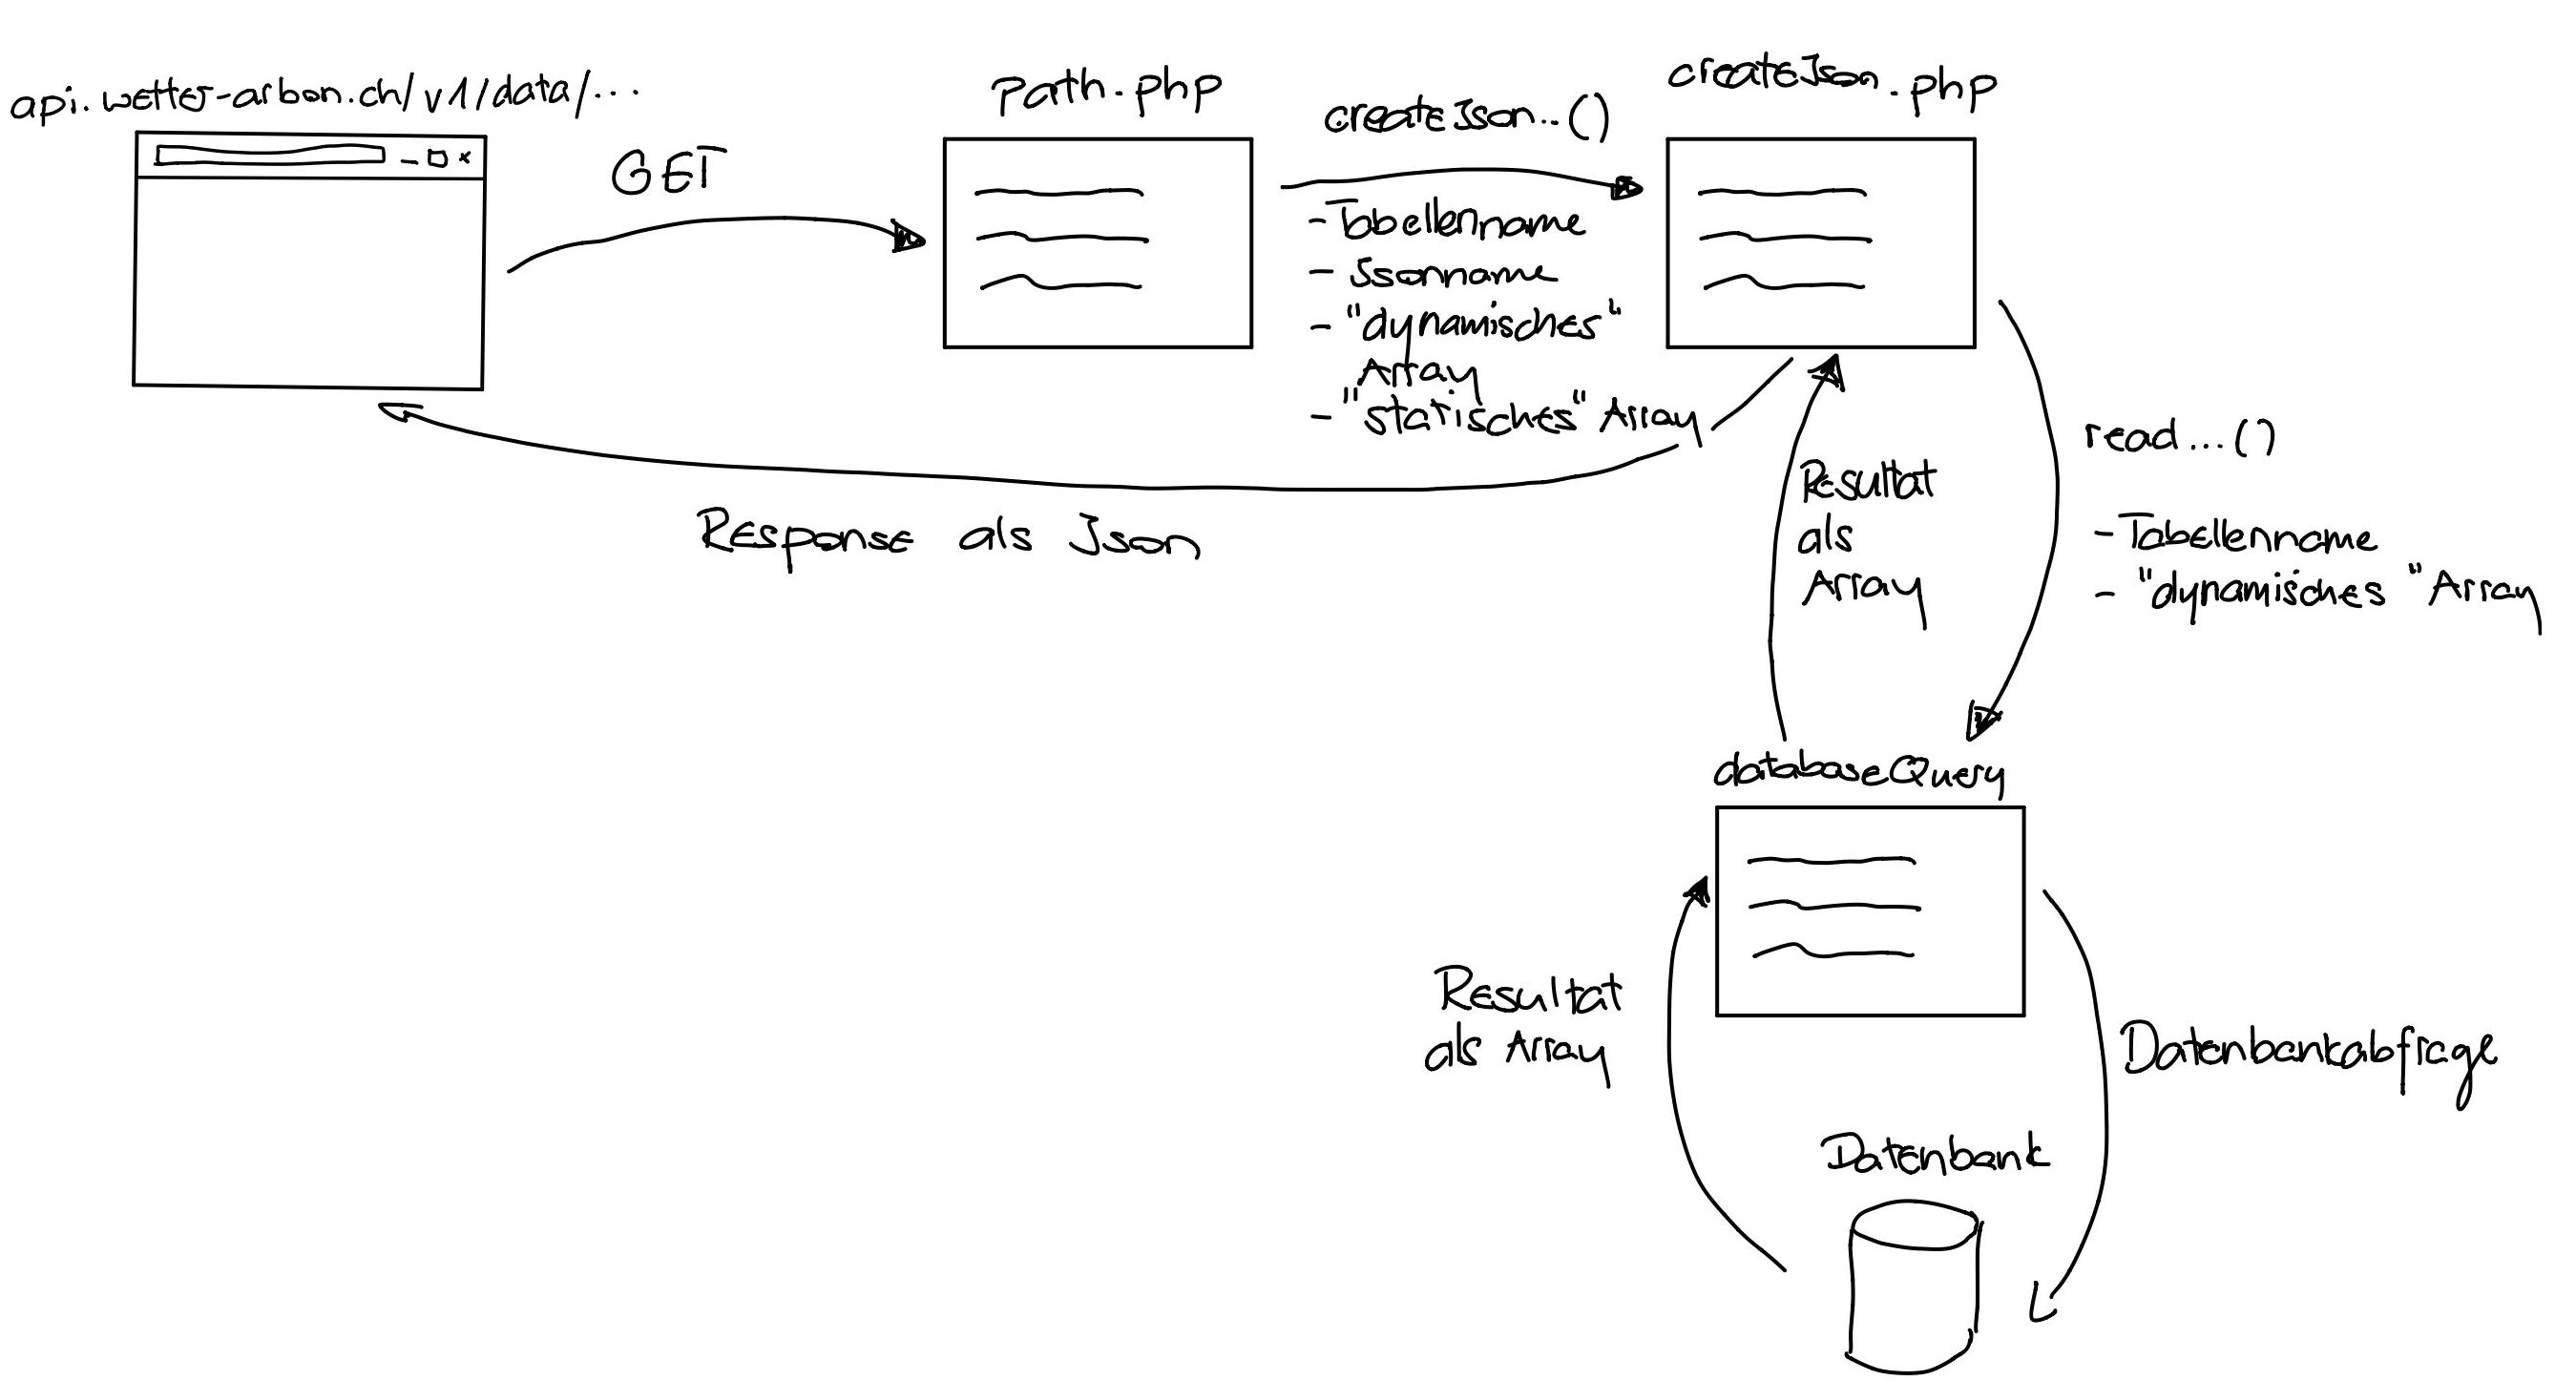
\includegraphics[width=\textwidth-2\fboxsep-2\fboxrule]{img/API_GET.jpg}}
	\centering
	\caption{Ablauf einer API GET-Abfrage}
	\label{img:APIFiles}
\end{figure}



\begin{lstlisting}[label=lst:path,caption=Beispiel Case zuweisung, language=php, style=php]
case "/v1/data/temperature":
	$table = "tblwettertransmitter";
	$requiredData = array(
		"value" => "temperature",
		"min"  	=> "min_daily_temperature",
		"max"   => "max_daily_temperature"
	);
	$dataJsonStatic = array(
	 "description"  => "Lufttemperatur",
	 "unit"  => "C"
	);
	$name = "temperature";
	createJsonMinMax($requiredData, $dataJsonStatic, $table, $name);
	break;
\end{lstlisting}



%% ############################################################################
%% Unterkapitel
%% ############################################################################
\subsection{API-Dokumentation}
postman vs. swagger.io
link zu Doku
%https://documenter.getpostman.com/view/4035921/api-wetter-arbon/RW1XMhBK

Das Verzeichnis V1 beinhaltet drei Unterverzeichnisse, data, misc und webcam. Im Verzeichnis Data wird das JSON der Sensoren aufgebaut, im Verzeichnis Webcam wird das JSON für die Webcam erstellt. Dies ist auch das einzige Verzeichnis welches nicht auf die Datenbank zugreift. Im Verzeichnis misc werden verschiedene Arten von Daten, welche von dritten abgegriffen werden verarbeitet. Nebst dem Verzeichnis, welches modular aufgebaut ist, enthalten auch die Dateien eine gewisse Struktur. Jedes Verzeichnis config enthält die folgenden vier Dateien.


Erfolgt eine GET-Abfrage eines Clients läuft dies gemäss Abb. \ref{img:APIFiles}  ab. Nach der GET-Abfrage wird das Routing anhand des URL Pfades im path.php vorgenommen. Im Case wird der entsprechende Funktionsaufruf mit den Parametern an das CreateJSON übergeben. Hier entsteht zum Schluss auch das JSON. Die Funktion CreateJson...() stellt das JSON nach der Datenbankabfrage read...() in der Datei databaseQuery.php her. Das JSON wird aus dem dynamischen Array, enthält die Messwerte, sowie dem statischen Array, enthält die Einheit und Beschreibung, zusammengesetzt und zurück gegeben.

Die Funktionen sind vom Aufbau her alle gleich. Der Unterschied besteht jedoch beim Aufbau des Json. Für einige Messwerte sind Maximal und Minimalwerte gewünscht. Andere Messwerte hingegen werden in verschiedene Einheiten umgerechnet, damit alle Benutzer die Messwerte auch interpretieren können.
